% 
%
\documentclass[12pt]{article}
% General packages
\usepackage{amsmath, graphicx, float, tabularx, booktabs}
% For coloring tables
%\usepackage[table]{xcolor}
% For adjusting margin size
\usepackage[margin=1in]{geometry}
% For setting bookmarks on pdf export
\usepackage[bookmarks,bookmarksopen,bookmarksdepth=2]{hyperref} 
\usepackage{cite}

% Image path location
\graphicspath{ {images/} }

%\rowcolors{2}{gray!25}{white}

\begin{document}

% Title infomation
\title{Linear Block Code Error Correction}
\author{Devin Trejo \tabularnewline devin.trejo@temple.edu }
\date{\today}
\maketitle

\section{Summary}
\label{sect:summary}


\section{Introduction}
\label{sect:intro}
\subsection{Hamming Linear Block Encoding/Decoding Theory}
The Hamming linear block code is a forward error detection and correction 
method where the original message is encoded to include more symbols to 
add redundancy to the original message. The process allows the receiver of
the message to check and attempt to correct errors introduced by a 
noisy communications channel. In this lab we will use a (6,3)~Hamming~code~(G)
which we will transform a 3-bit messages~($\vec{m}$) into 6-bit 
codewords~($\vec{x}$).

\begin{equation}
    \vec{x}=\vec{p}G \text{ where,}
    \label{eq:encoder}
\end{equation}

$$
    G=
    \begin{bmatrix}
        1 & 0 & 0 & 1 & 1 & 0 \\
        0 & 1 & 0 & 1 & 1 & 1 \\
        0 & 0 & 1 & 1 & 0 & 1
    \end{bmatrix} \quad
$$

On the receiving side we first take our received codeword~($\vec{r}$) and 
detect any errors in the received message. We do so by taking our 
codeword and checking it against a parity~matrix~(H). The resulting 
syndrome~($\vec{z}$) will point to the location of any errors in our 
transmitted data. Note that our linear block code produces a 
non-systematic codeword; meaning our message is not seperated into k message
bits and (n-k) parity bits. \cite{Balakrishnan2010} Instead our message is 
embedded within our error-correcting code to produce a unique codeword. 
%The 
%benefits of having a non-systematic codeword is that is maximizes the free 
%distance between each code so our error detection has increased performance. 

\begin{equation}
    \vec{z}=\vec{r}H \text{ where,}
    \label{eq:error_detector}
\end{equation}

$$
    H=
    \begin{bmatrix}
        1 & 1 & 0 \\
        1 & 1 & 1 \\
        1 & 0 & 1 \\
        1 & 0 & 0 \\
        0 & 1 & 0 \\
        0 & 0 & 1 \\
    \end{bmatrix}
$$

\begin{figure}[H]
    \centering
    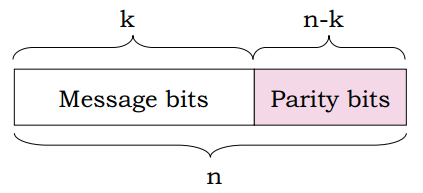
\includegraphics[width=2.5in]{systematic_encoded.PNG}
    \caption{Example of Systematic Encoding Formating
             \cite{Balakrishnan2010}}
\end{figure}

The error detector referenced by equation~\ref{eq:error_detector} is said to 
detect an error when the syndrome~($\vec{z}$) in non-zero. To correct any 
1-bit errors seen in the 6-bit received message requires we flip the bit
seen in the position referenced by the non-zero syndrome. For example,
if $\vec{z}=\begin{bmatrix} 0 & 1 & 0 \end{bmatrix}$ then we say corresponding
bit 2 in $\vec{r}$ needs to be flipped. 

After we have our codeword corrected ($\vec{r'}$), we can retrieve the 
original message ($\vec{p_r}$) by using a (3,6) decoding~matrix~(R). 
The decoding matrix reverses the steps taken by the generator~matrix~(G). 

\begin{equation}
    \vec{p_r}=\vec{r'}R \text{ where, }
    \label{eq:decoder}   
\end{equation}

$$
    R=
    \begin{bmatrix}
        1 & 0 & 0 \\
        0 & 1 & 0 \\
        0 & 0 & 1 \\
        0 & 0 & 0 \\
        0 & 0 & 0 \\
        0 & 0 & 0 \\
    \end{bmatrix}
$$

Finally we wish to look at the performance of this Hamming Linear Block code
encoder/decoder. The correction capacity for any given codeword is given by
equation~\ref{eq:correction_capacity} where t denotes the number of 
errors that are detectable and correctable. In some instances the receiver may
not be able to correct a received codeword but it is still detectable. 
The error detection~(e) is given by equation~\ref{eq:error_detection}.

\begin{equation}
    t=\lfloor{\frac{d_{min}-1}{2}}\rfloor
    \label{eq:correction_capacity}   
\end{equation}

\begin{equation}
    e={d_{min}-1}
    \label{eq:error_detection}   
\end{equation}

\subsection{Hamming Linear Block Encoding/Decoding Implementation}
For this lab we will transmit the message \textit{``EE is my avocation''} 
and set up a communication channel between a PIC32 Microchip MCU and 
Windows desktop over Ethernet. The Windows machine will run a Visual Basic 
application which will receive a message from the PIC32 server and 
introduce random errors to simluate errors that may be introduced
when transmitting over a noisy communications channel. VB client \
\textit{Client2 v16B} will introduce at most 1-bit in error within a given
message. VB Client \textit{Client3 v16} will introduce up to 10-bits in 
error. After we will setup our PIC32 MCU to receive a message from the VB 
client in order to perform error detection and correction using the Hamming 
linear block scheme.

To use a (6,3)~Hamming~code requires our individual messages to be 3-bits in
size. Therefore, we format our transmission string into messages 3-bits in 
size. We then will encode our message to produce 6-bit codewords. Since
our message is using characters within the standard ASCII table, the MSB in 
all characters will always be zero. Therefore, ignoring the MSB can now take 
our 7-bit ASCII character and break it up 3 individual bits. A combination 
of 3 characters will end up creating a perfect set to complete 7 packets 
we can send. 

$$
    \begin{array}{ccccc}
        'E' & = & [ 0 1 0 0 \quad 0 1 0 1] 
                & \rightarrow & [ 1 0 0 \quad 0 1 0 1] \\
        'E' & = & [ 0 1 0 0 \quad 0 1 0 1] 
                & \rightarrow & [ 1 0 0 \quad 0 1 0 1] \\
        '\text{\textvisiblespace }' & = & [ 0 1 0 0 \quad 0 0 0 0] 
                                    & \rightarrow
                                    & [ 1 0 0 \quad 0 0 0 0 ]
    \end{array}
$$

\begin{table}[H]
    \centering
    \begin{tabularx}{\textwidth}{|*{7}{>{\centering}X|}}
        \toprule
        100 & 010 & 110 & 001 & 011 & 000 & 000 \tabularnewline
        \midrule
        \multicolumn{1}{|c|}{\textit{\textbf{Packet0}}} & 
        \multicolumn{1}{|c|}{\textit{\textbf{Packet1}}} & 
        \multicolumn{1}{|c|}{\textit{\textbf{Packet2}}} & 
        \multicolumn{1}{|c|}{\textit{\textbf{Packet3}}} & 
        \multicolumn{1}{|c|}{\textit{\textbf{Packet4}}} & 
        \multicolumn{1}{|c|}{\textit{\textbf{Packet5}}} & 
        \multicolumn{1}{|c|}{\textit{\textbf{Packet6}}} \tabularnewline
        \bottomrule
    \end{tabularx}
    \caption{3-Bit Message Composition for First 3 Characters Before Encoding}
    \label{table:3-bit_message_no_encoding}   
\end{table}

Our overall message is 18 characters in length. Distributing our 18 
characters into 7 packets of length 3-bits produces 42 packets.
Those 42 packets will next be encoded using our (6,3)~Hamming 
linear block encoder to produce packets of 6-bits. Finally, we will 
pad each 6-bit packet with two leading zeros and send it as a 8-bit ASCII 
character. 

\section{Discussion}
\label{sect:discussion}

\bibliographystyle{plain}
\bibliography{../../../Mendeley/data_computer_communications}

\section*{Appendix}
\label{sect:appendix}
Main program runner source code available on GitHub:

\end{document}